% !TeX root = POSTER.tex
\documentclass[25pt, a0paper,
portrait,
% landscape,
margin=2mm, 
innermargin=2mm, 
blockverticalspace=7mm, %distance between upper and lower block
colspace=2mm, %distance between left and right block 
subcolspace=0mm]{tikzposter}
		
% -- Packages --------------------------------------------------------%
\usepackage{amsfonts,amssymb,amsmath,mathtools}
\usepackage{defcmlfont}
\usepackage{tikz,lipsum}

\usepackage[T1]{fontenc}
% \usepackage{lmodern}
% \usepackage[english]{babel}

\usetikzlibrary{positioning}
\usepackage{float}                           % for minipages at Polarization part
\usepackage{caption}                         % no "Figure" in caption
\captionsetup[figure]{labelformat=empty}

\usepackage{psfrag}

% Load figures command: \inputfig [htb]{fig_dir}{fig_label}
\newcommand*{\inputfig}[3][htb]{{
    \def\fps@figure{#1}
    \def\DIR{#2}
    \def\LABEL{#3}
    \graphicspath{{\DIR/}}
    \psfrag{sm}[c][c]{\small \textsc{Scan me}}


\includegraphics[width=0.03\textwidth]{QRcode_ACoM.eps}
}}

\usepackage{fontawesome}
\usepackage{bm}
\usepackage{bigints}
\usepackage{relsize}

\usepackage{accents}

\usepackage{lipsum} 

\usepackage{babel}
\usepackage{hyperref}
\usepackage{cleveref}

\usepackage{mdframed}

\usepackage{xcolor}

% double int with circle \oiint
\usepackage{esint}

\usepackage{cancel}

% -- Commands --------------------------------------------------------%
% \newcommand{\wall}{\text{w}}
% \newcommand{\interf}{\text{i}}
% \newcommand{\phase}{k}	
% \newcommand{\liquid}{\ell}
% \newcommand{\steam}{g}
% \newcommand{\out}{\text{out}}
% \newcommand{\tr}{{\mathsf T}}
\newcommand{\WA}{\prescript{\mathcal{W}}{}{\!\!\!\mathcal{A}}}
\newcommand{\WAz}{\prescript{\mathcal{W}}{}{\!\!\!\mathcal{A}}(z)}
\newcommand{\WApz}{\prescript{\mathcal{W}}{}{\!\!\!\mathcal{A}}'(z)}
\newcommand{\WAxx}{\prescript{\mathcal{W}}{}{\!\!\!\mathcal{A}}(x_1,x_2)}

\newcommand{\WAsigma}{\prescript{\prescript{\mathcal{W}}{}{\!\!\!\mathcal{A}}}{}{\!\sigma}}
\newcommand{\WABsigma}{\prescript{\prescript{\mathcal{W}}{}{\!\!\!\mathcal{A}}}{}{\!\boldsymbol{\sigma}}}

% Mathematic sets
\newcommand{\mbR}{\mathbb{R}}
\newcommand{\mbC}{\mathbb{C}}

% mathcals
\newcommand{\mcA}{\mathcal{A}}
\newcommand{\mcB}{\mathcal{B}}
\newcommand{\mcC}{\mathcal{C}}
\newcommand{\mcD}{\mathcal{D}}
\newcommand{\mcE}{\mathcal{E}}
\newcommand{\mcO}{\mathcal{O}}
\newcommand{\mcS}{\mathcal{S}}
\newcommand{\mcT}{\mathcal{T}}
\newcommand{\mcV}{\mathcal{V}}
\newcommand{\mcW}{\mathcal{W}}

\newcommand{\mcK}{\mathcal{K}}
\newcommand{\mcM}{\mathcal{M}}
\newcommand{\mcZ}{\mathcal{Z}}

\newcommand{\bigoiintsss}{\mathlarger{\mathlarger{\varoiint}}}
\newcommand{\bigoiintssss}{\mathlarger{\varoiint}}

\newcommand{\Kipc}{\mathcal{K}^{c}}
\newcommand{\Kipcz}{\mathcal{K}^{c}(z)}

% -- Title, Author, Institute --------------------------------------------------------%
% \title{
% \begin{minipage}{0.22\textwidth}
% 	
\includegraphics[width=1.02\textwidth]{./floats/logos/siam_siamcse23.eps}
% \end{minipage}
% \hfill
% \begin{minipage}{0.46\textwidth}
% 	\begin{flushleft}
% 		{\bfseries Next-generation all-solid-state battery}
% 	\end{flushleft}
% 	% \author{\underline{Tuan Vo}$^{\text{a,b}\,\dagger}$, Claas Hüter$^{\text{b}}$, Stefanie Braun$^{\text{a}}$, Manuel Torrilhon$^{\text{a}}$}
% 	% {\normalsize \underline{Tuan Vo}$^{\text{a,b}\,\dagger}$, Claas Hüter$^{\text{b}}$, Stefanie Braun$^{\text{a}}$, Manuel Torrilhon$^{\text{a}}$}
% \end{minipage}
% \hfill
% \begin{minipage}{0.22\textwidth}
% 	% \begin{flushleft}
% 		
\includegraphics[width=1.02\textwidth]{./floats/logos/rwth_acom_en_cmyk_fzj_gap.eps}
% 	% \end{flushleft}
% \end{minipage}
% }
\title{\scshape Next-generation all-solid-state battery (\#ASSB)}
\author{
	\underline{Tuan Vo}$^{\text{a,b}\,\dagger}$, Claas Hüter$^{\text{b}}$, Stefanie Braun$^{\text{a}}$, Manuel Torrilhon$^{\text{a}}$\\
\normalsize vo@acom.rwth-aachen.de}
\author{\underline{Tuan Vo}$^{\text{a,b}\,\dagger}$, Claas Hüter$^{\text{b}}$, Stefanie Braun$^{\text{a}}$, Manuel Torrilhon$^{\text{a}}$}
\institute{\large
$\prescript{a}{}{}$Department of Mathematics, Applied and Computational Mathematics (ACoM), 
RWTH Aachen University, Schinkelstraße 02, 52062 Aachen, Germany\\
$\prescript{b}{}{}$Institute of Energy and Climate Research (IEK-2), 
Forschungszentrum Jülich, Wilhelm-Johnen-Straße, 52428 Jülich, Germany
}

% \titlegraphic{
\includegraphics[height=6cm]{./figs/FZJ_only.pdf} \hfill 
\includegraphics[height=6cm]{./figs/rwth_mathcces_bild_rgb_only.pdf} }
% \titlegraphic{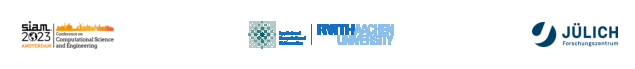
\includegraphics[width=0.3\textwidth]{./floats/logos/rwth_acom_en_cmyk_siamcse23_fzj_gap.eps}}

% \renewcommand{\familydefault}{\sfdefault} % Change font family

\bibliographystyle{plain}

\newcommand{\newcaption}[2]{\parbox{#1}{\centering{\small \it #2\par}}\normalsize}

% -- Predefined Colors and Themes ---------------------- %
% Choose THEME:  Default, Basic, Rays, Simple, Envelope, Wave, Board, Autumn, Desert,
% Explanation THEME: Default(gray+blueBC), Basic(green light), Rays(blue), 
% Simple(red), Envelope(Bluefancy), Wave(Bluefancy2), Board(Bluelight), Autumn(squarebox+bluebrown), Desert(squarebox+bluebrown2),
\usetheme{Default}

\useblockstyle[titleinnersep=0.7mm]{Default}    % change default parameter for title inner sep
% Choose COLOR STYLE:  Default, Blue, BlueGray, BlueOrange, BlueViolet, DarkBlue, GrayBlue, GrayLightblue, GrayRed, Green, GreenOrange, YellowRed
%\definecolor{main}{HTML}{0080FF}
%\definecolor{sub}{HTML}{8CDBFF}
%\usecolorstyle[colorOne=sub, colorTwo=main]{Default}
% ---------------------------------------------------------------------------------------------------------------- %
\begin{document}
% Title block
\maketitle[width=800mm]
% ---------------------------------------------------------------------------------------------------------------- %
\block{\bfseries Mathematical modelling for the next-generation All-solid-state batteries: Nucleation $\text{(SE|SSE)}^{\!(*)}$-interface}
{
	\begin{minipage}{0.56\textwidth}
		\begin{minipage}{0.5\textwidth}
			\begin{mdframed}
				\textbf{Rechargeable Lithium-ion battery} (LIB)
				is at the heart of every electric vehicle (EV), portable electronic device,
				and energy storage system \cite{vo2018}. 
				Nowadays, LIBs enable human life more efficient 
				and help to solve global environment issues thanks to EVs' zero emission.
				However, conventional LIB (c-LIB) is sensible to temperature and pressure, 
				hence, flammable and explosive, which is \colorbox{pink}{undesirable}. 
				This bottleneck is
				mainly due to \colorbox{cyan}{liquid-based electrolyte} found in c-LIBs.
			\end{mdframed}
		\end{minipage}
		%
		\begin{minipage}{0.49\textwidth}
			\begin{mdframed}
				\textbf{All-solid-state battery} (ASSB) is 
				one of promising candidates to overcome bottlenecks of c-LIBs. 
				Thanks to \colorbox{cyan}{solid-state electrolyte} (SSE),
				ASSB is highly stable towards temperature and pressure. 
				Nevertheless, Li-metal dendrite 
				triggered at (SE|SSE)-interface \cite{kim2022}
				is the main drawback of ASSB
				since these dendritic threads
				extrapolate into SSE grain boundary network, 
				causing crevice, degradation of ionic conductivity,
				and the probability of short-circuit, which is \colorbox{pink}{unfavorable}.
			\end{mdframed}
		\end{minipage}
		%
		\begin{mdframed}
			\textbf{Next-generation All-solid-state battery} (ng-ASSB)
			with a consideration of \colorbox{cyan}{nucleation criterion} defined by
			\begin{align*}
				a_{\text{Griffith}} := a^{*} = \arg\min_{a\in\mathbb{R}}{\bigintsss\!\!\!\!\!\!\bigintsss\!\!\!\!\!\!\bigintsss_{\Omega} f(a,\bm{u},\theta;\lambda,\mu,\bm{d}^{R}\otimes\bm{d}^{R}) \, d\Omega - \bigintsss\!\!\!\!\!\!\bigintsss_{\Gamma} f(a;\gamma) \, d\Gamma}\Bigg|_{\bm{u}^{(s)}}
			\end{align*}
			where 
			$\Bu$ displacement field, 
			$\theta$ temperature field, 
			$a$ crevice length,
			$\lambda, \mu$ Lam\'{e} constants,
			$\Bd^{R}\otimes\Bd^{R}$ embedded misorientation structural tensor,
			and 
			$\gamma$ cracking-surface energy density,
			\colorbox{pink}{can help} to improve ASSB performance.
		\end{mdframed}
	\end{minipage}%
	\hfill
	\begin{minipage}{0.44\textwidth}
		\begin{center}
			\inputfig{floats/routine_woTV_spectral}{routine_woTV_spectral}
		\end{center}
	\end{minipage}
	\vspace{-0.3cm}
}
% ---------------------------------------------------------------------------------------------------------------- %
\begin{columns}
	\column{0.34}{
		\block{Interface Analysis}{
			\textbf{Interface} between solid electrode and solid-state electrolyte (SE|SSE) 
			taking place at space charge layer (SCL) \cite{braun2015}
			found in ASSBs 
			critically exhibits mechanical and electrochemical instability \cite{hueter2017}. 
			This evidence points directly to the fact that 
			the soft metallic li anode 
			is erroneously prone to triggering dendrites, 
			under cycles of electric charge \& discharge \cite{kim2022}.
			\begin{center}
				\inputfig{floats/maxshear_9figs_456}{maxshear_9figs_456}
			\end{center}
			\underline{Distribution}:\! 
			ana. max. shear stress $\WAsigma^{\Pi}_{x_1x_2}$ around crack tip $a_{c}$.
		}
	}
	% ---------------------------------------------------------------------------------------------------------------- %
	\column{0.338}
	\block{Next-generation All-solid-state battery}
	{
		\textbf{Nucleation} criterion governs the instable (SE|SSE)-interface \cite{hueter2017}
		\begin{center}
			\inputfig{floats/dendrite_pdirection_battonly}{dendrite_pdirection_battonly}
		\end{center}
		$\checkmark$ \textbf{Thermodynamic consistency} is satisfied, followed by \cite{braun2015}.\\
		$\checkmark$ \textbf{Closure} $\bar{\Omega}$ is fulfilled by 15 moments, followed by \cite{torrilhon2016}.
	}
	% ---------------------------------------------------------------------------------------------------------------- %
	\column{0.322}
	\block{Embedded structural-tensor in SSE}
	{
		\textbf{Polycrystalline} garnet-type SSE \cite{kim2022}
		such as LLZO 
		exhibit grain boundary network, 
		and grains with variation of $\left\{ \text{size, shape} \right\}$
		under microscopic observation.
		Hence, this microstructure is
		potentially prone to
		nuances of destruction.
		% ceramic-like materials.
		\begin{align*}
			\BM = \Bd^{R}_{G_1} \otimes \Bd^{R}_{G_2}
			\quad 
			\text{given by}
			\quad
			\mathbb{G} := \left\{ \BQ_{||_{\Bd}}, \BQ_{\bot_{\Bd}}  \right\} \subset \mathcal{O}(3).
		\end{align*}
		\begin{center}
			\inputfig{floats/dendrite_2parts_nospl_split}{dendrite_2parts_nosample_split}
		\end{center}
		Consequentially, dendrites contribute to 
		degradation of ionic conductivity
		and tiny-cracks tracing along grain boundaries.
	}
\end{columns}
% ---------------------------------------------------------------------------------------------------------------- %
\block{Nucleation interface: Taking place at the critical dendritic interface}
{
	\begin{minipage}{0.43\textwidth}
		\begin{mdframed}
			\underline{Coupled fields}: Displacement field $\Bu$ and temperature field $\theta$; structural tensor $\BM$
			\begin{align*}
				\Bu:
				\begin{cases}
					\Omega \times \mathbb{R}_{+} \rightarrow \mathbb{R}^3, \\
					(\Bx,t) \mapsto \Bu(\Bx,t),
				\end{cases}
				%
				\theta:
				\begin{cases}
					\Omega \times \mathbb{R}_{+} \rightarrow \mathbb{R}, \\
					(\Bx,t) \mapsto \theta(\Bx,t),
				\end{cases}
				%
				\BM^{\{RR,RE\}}_{i=1,\dots,N}:
				\begin{cases}
					% \left( 
					\Bd^{R}_{\text{\tiny Grain i}} \otimes \Bd^{R}_{\text{\tiny Grain i}} 
					% \right)
					% \!\!\big|_{\tiny{i=1,\dots,N}}
					\\
					\Bd^{R}_{\text{\tiny Grain i}} \otimes \Bd^{E}
				\end{cases}
			\end{align*}
			Governing conservation equations
			\begin{align*}
				\frac{d}{dt} \int_{\Omega}(\cdot)\ d\Omega = \int_{\Omega}(\cdot)^{\text{\tiny action}}\ d\Omega 
				+ \int_{\partial\Omega}(\cdot)^{\text{\tiny action}}\ d\partial\Omega  
				+ \int_{\Omega}(\cdot)^{\text{\tiny production +/-}}\ d\Omega
			\end{align*}
			$\rho(\Bx,t)$ is mass density per unit volume (puv); 
			$\Bb(\Bx,t)$ body force puv; 
			$\Bv(\Bx,t)$ velocity; 
			$e(\Bx,t)$ internal energy puv; 
			$\Bq(\Bx,t)$ heat flux; 
			$r(\Bx,t)$ heat source puv; 
			$\Bsigma$ Cauchy stress and 
			$\Bvarepsilon$ infinitesimal strain.
			%
			Helmholtz energy functional 
			\begin{align*}
				a_{\text{Griffith}} := a^{*} = \arg\min_{a\in\mathbb{R}}{\bigintsss\!\!\!\!\!\!\bigintsss\!\!\!\!\!\!\bigintsss_{\Omega} f(a,\bm{u};\lambda,\mu,\bm{d}\otimes\bm{d}) \, d\Omega - \bigintsss\!\!\!\!\!\!\bigintsss_{\Gamma} f(a;\gamma) \, d\Gamma}\Bigg|_{\bm{u}^{(s)}}
			\end{align*}
			Governing PDE
			\begin{align*}
				a_{\text{Griffith}} := a^{*} = \arg\min_{a\in\mathbb{R}}{\bigintsss\!\!\!\!\!\!\bigintsss\!\!\!\!\!\!\bigintsss_{\Omega} f(a,\bm{u};\lambda,\mu,\bm{d}\otimes\bm{d}) \, d\Omega - \bigintsss\!\!\!\!\!\!\bigintsss_{\Gamma} f(a;\gamma) \, d\Gamma}\Bigg|_{\bm{u}^{(s)}}
			\end{align*}
			abc
		\end{mdframed}
		\begin{minipage}{0.5\textwidth}
			\begin{mdframed}
				\textbf{Strain energy}: 
				Interface between solid electrode and solid-state electrolyte (SE|SSE) 
				taking place at space charge
				\begin{align*}
					\bigintsss\!\!\!\!\!\!\bigintsss\!\!\!\!\!\!\bigintsss_{\Omega}
					f(a,\bm{u};\lambda,\mu,\bm{d}\otimes\bm{d}) \, d\Omega 
				\end{align*}
			\end{mdframed}
		\end{minipage}
		\hfill 
		\begin{minipage}{0.49\textwidth}
			\begin{mdframed}
				\textbf{Surface energy}: 
				Interface between solid electrode and solid-state electrolyte (SE|SSE) 
				taking place 
				\begin{align*} 
					\bigintsss\!\!\!\!\!\!\bigintsss_{\Gamma} f(a;\gamma) \, d\Gamma
				\end{align*}
			\end{mdframed}
		\end{minipage}
		%
		\begin{mdframed}
			Therefore, the governing problem of dendritic nucleation at (SE|SSE) takes the form
			\begin{align*}
				 & 
				\cancel{\partial_{t}\bm{u}}
				+
				\nabla \cdot
				\Big(
				\accentset{\scriptstyle 4}{\mathbb{C}}^{f_{\text{alocation}}(\lambda,\mu,\Bd^{R}_{G_i, i=1,\dots,N},\Bd^{E};\Bx)}
				:\nabla\Bu^{(s)}
				\Big)
				+ \rho\Bb
				= -\rho\nabla V_{e}, \\
				%--------------------------------
				\text{s.t.}\ \
				 & 
				a_{\text{Griffith}} := a^{*}
				= \arg\min_{a\in\mathbb{R}}
				{
					\bigintsss\!\!\!\!\!\!\bigintsss\!\!\!\!\!\!\bigintsss_{\Omega}
					f(a,\bm{u},\theta;\lambda,\mu,\bm{d}\otimes\bm{d}) \, d\Omega
					- 
					\bigintsss\!\!\!\!\!\!\bigintsss_{\Gamma} f(a;\gamma) \, d\Gamma
				}
				\Big|_{\bar{\bm{u}}}
			\end{align*}
			where
		\end{mdframed}
	\end{minipage}
	\hfill
	\begin{minipage}{0.54\textwidth}
		\begin{minipage}{0.7\textwidth}
			\begin{mdframed}
				\underline{Boundary conditions}
				\begin{center}
					\inputfig{floats/structuraltwofields}{structuraltwofields}
				\end{center}
			\end{mdframed}
			\begin{mdframed}
				% The set of boundary conditions is likewise the path of the pressure-centric dendritic crack.\\
				\begin{center}
					\inputfig{floats/routine_woTV_numa_one}{routine_woTV_numa_one}
				\end{center}
				\underline{Comparison}: Analytical vs. Numerical solutions
				\begin{center}
					\inputfig{floats/comparison_ana_numa}{comparison_ana_numa}
				\end{center}
			\end{mdframed}
		\end{minipage}
		\hfill 
		\begin{minipage}{0.3\textwidth}
			\begin{mdframed}
				FEM: Strain energy density
				\vspace{0.1cm}
				\inputfig{floats/griffith_flowchart_circle_formula}{griffith_flowchart_circle_formula}
				abc\\
				abc
			\end{mdframed}
		\end{minipage}
		%
		\begin{mdframed}
			\underline{Analysis}: Airy-Westergaard function used for stress analysis:
			(i) max. shear stress and (ii) principal stresses
			\begin{align*}
				\WA:
				\begin{cases}
					\mbC\to\mbC, \\
					% \displaystyle
					z \mapsto \WAz:=
					\Re(\bigoiintssss_{\Gamma} \mcK^{(\star)}\,dz )
					+ x_2\,
					\Im(\bigointsss_{\Gamma} \mcK^{(\star)}\,dz ),
				\end{cases}
				\mcK^{(\star)}:
				\begin{cases}
					\mbC \to \mbC, \\
					z \mapsto 
					\mcK^{(\star)}:=
					- p_{h} + p_{h}/\sqrt{1 - a^2/z^2},\
				\end{cases}
			\end{align*}
			where $a$ the crevice length, $p_{h}$ pressure at the opening crevice on dendritic interface, and $\forall \, \{p_{h},a\}\in\mbR_{+}$.
		\end{mdframed}
		%
		\begin{mdframed}
			\underline{Numerics $\rightarrow$ FEM}:
			element matrix $\BK^{e}$
			approx. by \textit{Gauss quadrature}; 
			indices imply \textit{$4+2=6$ \textit{for}-loop}:
			\begin{align*}
				K^{\stackrel{\alpha\beta}{e\ \ }}_{ik} = 
				\int_{\Omega^{\xi}}
				\left(
				\mathcal{L}^{\alpha}_{1} \ \mathbb{C}_{i1k1}^{f^{GL}}(\Bx) \ \mathcal{R}^{\beta}_{1} +
				\mathcal{L}^{\alpha}_{1} \ \mathbb{C}_{i1k2}^{f^{GL}}(\Bx) \ \mathcal{R}^{\beta}_{2} +
				\mathcal{L}^{\alpha}_{2} \ \mathbb{C}_{i2k1}^{f^{GL}}(\Bx) \ \mathcal{R}^{\beta}_{1} +
				\mathcal{L}^{\alpha}_{2} \ \mathbb{C}_{i2k2}^{f^{GL}}(\Bx) \ \mathcal{R}^{\beta}_{2}
				\right)
				\det(\BJ) \ d\Omega^{\xi}
			\end{align*}
			where $\mathcal{L}^{\alpha}_{j}$ and $\mathcal{R}^{\beta}_{l}$ are gradients of basis functions at node $\alpha^{th}$ and $\beta^{th}$, respectively.
		\end{mdframed}
	\end{minipage}
	\vspace{-0.4cm}
}
% ----------------------------------------------------------------------------------------------------------------
\begin{columns}
	\column{0.14}
	% ---------------------------------------------------------------------------------------------------------------- %	
	\block{Contact}{
		% {
		% 		\raggedleft
		% 		\begin{tikzpicture}
		% 			\node (qrcode) {\inputfig{floats/QRcode_ACoM}{QRcode_ACoM}};
		% 			\node[left= 0mm of qrcode.north west, yshift=-15mm] {Tuan Vo};
		% 			% \node[left= 0mm of qrcode.north west, yshift=-40mm] {Applied and Computational Mathematics (ACoM)};
		% 			% \node[left= 0mm of qrcode.north west, yshift=-55mm] {RWTH Aachen University};
		% 			\node[left= 0mm of qrcode.north west, yshift=-30mm] {vo@acom.rwth-aachen.de};
		% 		\end{tikzpicture}
		% 	}
		\begin{center}
			\inputfig{floats/QRcode_ACoM_Email}{QRcode_ACoM_Email}
		\end{center}
	}
	\column{0.86}
	%---------------------------------------------------------------------------------------------------------------- %	
	\block{References}{
		\vspace*{-3em}
		\renewcommand{\refname}{~}
		\vspace{-0.4cm}
		\begin{thebibliography}{2}
			\bibitem{vo2018}
			\textbf{T.Vo},
			\!\!
			\emph{Modeling\! the\! swelling\! phenomena\! of\! li-ion\! batt.\!
				cells\! based\! on\! a\! numerical\! chemo-mech.\! coupled\! approach}.
			MA, Robert Bosch Battery Systems GmbH, \textbf{2018}.
			
			\bibitem{braun2015}
			\textbf{S.Braun},\! C.Yada\! and A.Latz,
			\!\!\!\!
			\emph{Thermodynamically\! consistent\! model\! for\!
				Space-Charge-Layer\! formation\! in\! a\! solid\! electrolyte}.
			Jr.\! Phys.\! Chem.,\! 119,\! 22281-22288,\! \textbf{2015}.
			
			\bibitem{hueter2017}
			\textbf{C.Hüter}, S.Fu, M.Finsterbusch, E.Figgemeier, L.Wells, and R.Spatschek,
			\emph{Electrode-electrolyte interface stability in solid state electrolyte system:
				influence of coating thickness under varying residual stresses}. 
			AIMS Materials Science, 4(4):867-877, \textbf{2017}.
			
			\bibitem{torrilhon2016}
			\textbf{M.Torrilhon}. 
			\emph{Modeling nonequilibrium gas flow based on moment equations}.
			Annual Review of Fluid Mechanics, 48(1):429-458, \textbf{2016}.
			
			\bibitem{kim2022}
			\textbf{S.Kim}, 
			J.S.Kim, L.Miara, Y.Wang, S.K.Jung, S.Y.Park, Z.Song, 
			H.King, M.Badding, J.M.Chang, V.Roev, G.Yoon, R.Kim, J.H.Kim, K.Yoon, D.Im, and K.Kang,
			\emph{High-energy and durable li metal batt. using garnet-type
				solid electrolytes with tailored li-metal compatibility}.
			Nature Communications, 13(1):1883, \textbf{2022}.
			% $(*)$ (Solid electrode | Solid-state electrolyte)
		\end{thebibliography}
		\vspace{-0.8cm}
	}
\end{columns}
% ----------------------------------------------------------------------------------------------------------------
\block{}
{
	\vspace{-0.6em}
	\begin{minipage}{0.2\textwidth}
		\begin{center}
			
\includegraphics[width=0.99\textwidth]{./floats/logos/siam.eps}
		\end{center}
	\end{minipage}
	\hfill
	\begin{minipage}{0.2\textwidth}
		\begin{center}
			
\includegraphics[width=0.45\textwidth]{./floats/logos/siamcse23.eps}
		\end{center}
	\end{minipage}
	\hfill
	\begin{minipage}{0.2\textwidth}
		\begin{center}
			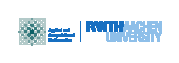
\includegraphics[width=0.85\textwidth]{./floats/logos/acomrwth.eps}
		\end{center}
	\end{minipage}
	\hfill
	\begin{minipage}{0.2\textwidth}
		\begin{center}
			
\includegraphics[width=0.5\textwidth]{./floats/logos/fzj.eps}
		\end{center}
	\end{minipage}
	\vspace{-0.6em}
}
\end{document}
% ----------------------------------------------------------------------------------------------------------------